\chapter{Σύγκριση Αντιστοίχισης Αλγορίθμου Θεωρίας Παιγνίων με Αλγορίθμους Μηχανικής Μάθησης}

Στο δεύτερο, αυτό κομμάτι της διπλωματικής εργασίας, θα συγκρίνουμε τον Αλγόριθμο Θεωρίας Παιγνίων, που παρουσιάσαμε στο προηγούμενο κεφάλαιο, με άλλους αλγορίθμους που χρησιμοποιούνται σε παρόμοιες περιπτώσεις. Συγκεκριμένα θα μελετήσουμε την συμπεριφορά αλγορίθμων Μηχανικής Μάθησης - Ενισχυτικής Μάθησης, αλλά θα χρησιμοποιήσουμε και ως σημείο αναφοράς τον αλγόριθμο τυχαίας αντιστοίχισης, ώστε να αποφανθούμε για τα οφέλη που μας προσφέρουν οι υπόλοιποι αλγόριθμοι.

Η Ενισχυτική Μάθηση (Reinforcement Learning, RL) περιλαμβάνει μια ποικιλία αλγορίθμων που έχουν σχεδιαστεί για να μαθαίνουν τις βέλτιστες πολιτικές επιλογής ενεργειών μέσω αλληλεπιδράσεων με ένα περιβάλλον. Οι βασικές μέθοδοι βασισμένες σε τιμές περιλαμβάνουν τους αλγόριθμους Q-Learning και SARSA (State-Action-Reward-State-Action). Το Q-Learning είναι ένας εκτός πολιτικής αλγόριθμος που ενημερώνει επαναληπτικά τις τιμές Q για να εκτιμήσει την αναμενόμενη χρησιμότητα των ενεργειών σε δεδομένες καταστάσεις, ανεξάρτητα από τις ενέργειες του πράκτορα (ατόμου - κόμβου). Στοχεύει να μάθει την βέλτιστη πολιτική μεγιστοποιώντας τη συνολική ανταμοιβή με την πάροδο του χρόνου. Αντίθετα, το SARSA είναι ένας εντός πολιτικής αλγόριθμος που ενημερώνει τις τιμές Q βάσει των πραγματικών ενεργειών που λαμβάνονται από την πολιτική, αντί της μέγιστης δυνατής ενέργειας. Αυτό επιτρέπει στο SARSA να ενσωματώνει άμεσα τα αποτελέσματα της τρέχουσας πολιτικής του πράκτορα στη διαδικασία μάθησης. \lcite{reinforcement_overview_classification}

Τα Βαθειά Q-Δίκτυα (Deep Q-Networks - DQN) επεκτείνουν το Q-Learning ενσωματώνοντας βαθιά νευρωνικά δίκτυα, επιτρέποντας τη διαχείριση χώρων καταστάσεων υψηλής διάστασης. Τα Βαθειά Q-Δίκτυα χρησιμοποιούν αναπαραγωγή εμπειριών για να αποθηκεύουν και να επαναχρησιμοποιούν παλαιότερες εμπειρίες, βοηθώντας στη διακοπή της συσχέτισης μεταξύ διαδοχικών βημάτων μάθησης και βελτιώνοντας την αποδοτικότητα της εκπαίδευσης. Επιπλέον, τα Βαθειά Q-Δίκτυα χρησιμοποιούν ένα δίκτυο στόχου για να παρέχουν σταθερούς στόχους τιμών Q, μειώνοντας έτσι τα προβλήματα αστάθειας που προκύπτουν κατά την εκπαίδευση νευρωνικών δικτύων. \lcite{reinforcement_overview_classification}

Στην δική μας περίπτωση, οι τεχνικές Ενισχυτικής Μάθησης χρησιμοποιούνται όλο και περισσότερο στις λειτουργίες αντιστοίχισης σε διάφορους τομείς, όπως συστήματα συστάσεων, διαδικτυακή διαφήμιση και κατανομή πόρων. Σε αυτές τις εφαρμογές, οι αλγόριθμοι Ενισχυτικής Μάθησης, βελτιστοποιούν τη διαδικασία αντιστοίχισης μαθαίνοντας από τις αλληλεπιδράσεις με το περιβάλλον. Για παράδειγμα, στα συστήματα συστάσεων, οι πράκτορες Ενισχυτικής Μάθησης βελτιώνουν διαδοχικά τις προτάσεις τους λαμβάνοντας υπόψη την ανατροφοδότηση των κόμβων και ενημερώνοντας τις πολιτικές τους για τη μεγιστοποίηση της μακροπρόθεσμης εμπλοκής και ικανοποίησης των κόμβων. \lcite{Afsar2022}

Σε αντίστοιχη περίπτωση, μπορούμε να χρησιμοποιήσουμε τέτοιους αλγορίθμους για την αντιστοίχιση των κόμβων μας με τους εξυπηρετητές. Μέσω της Ενισχυτικής Μάθησης, οι κόμβοι λαμβάνουν αμοιβές ανάλογα με την ενέργεια που επιλέγουν κάθε φορά και έπειτα από συγκεκριμένο αριθμό επαναλήψεων, ο κάθε κόμβος επιλέγει την βέλτιστη ενέργεια με βάση τις αμοιβές που έχει συλλέξει. 

\section{Περιγραφή Αλγορίθμων Ενισχυτικής Μάθησης}

Για την εξερεύνηση και επιλογή ενεργειών από τους κόμβους θα χρησιμοποιήσουμε την αλγοριθμική τεχνική Ανώτατου Ορίου Εμπιστοσύνης (Upper Confidence Bound - UCB). Ο αλγόριθμος Ανώτατου Ορίου Αυτοπεποίθησης είναι μια στρατηγική που χρησιμοποιείται στη ενισχυτική μάθηση και στα προβλήματα πολλαπλών ένοπλων ληστών (multi-armed bandit) για να εξισορροπήσει αποτελεσματικά την εξερεύνηση και την εκμετάλλευση. Σε αντίθεση με απλές μεθόδους όπως ο αλγόριθμος ε-άπληστος (ε-greedy), ο Ανώτατου Ορίου Αυτοπεποίθησης επιλέγει ενέργειες με βάση τόσο τις εκτιμώμενες ανταμοιβές όσο και την αβεβαιότητα σε αυτές τις εκτιμήσεις. Δίνοντας προτεραιότητα σε ενέργειες με μεγαλύτερη αβεβαιότητα, ο Ανώτατου Ορίου Αυτοπεποίθησης εξερευνά συστηματικά λιγότερο δοκιμασμένες επιλογές, διασφαλίζοντας ότι ο αλγόριθμος συγκεντρώνει επαρκείς πληροφορίες για όλες τις πιθανές ενέργειες. Αυτή η προσέγγιση βοηθά στην πιο αξιόπιστη αναγνώριση της βέλτιστης ενέργειας με την πάροδο του χρόνου. Η μεθοδική μέθοδος του Ανώτατου Ορίου Αυτοπεποίθησης για την εξισορρόπηση της εξερεύνησης και της εκμετάλλευσης τον καθιστά ιδιαίτερα χρήσιμο σε σενάρια όπου η κατανόηση των υποκείμενων κατανομών ανταμοιβής είναι κρίσιμη για την μακροπρόθεσμη επιτυχία. \lcite{sutton2018ucb}

Στην περίπτωσή μας, ακολουθούμε την εξής διαδικασία: Αρχικά, κάθε κόμβος δεν ανήκει σε κανέναν εξυπηρετητή. Σε κάθε επανάληψη, κάθε κόμβος συλλέγει τις ενέργειες που μπορεί να επιλέξει να εκτελέσει. Στην συνέχεια εφαρμόζει τον κανόνα επιλογής ενέργειας του Αλγορίθμου Ανώτατου Ορίου Αυτοπεποίθησης για να επιλέξει την βέλτιστη ενέργεια σύμφωνα με τα μέχρι τώρα δεδομένα του (προφανώς αρχικά δεν έχει λάβει κάποια ανατροφοδότηση από το περιβάλλον του). Ο κανόνας επιλογής ενέργειας του αλγορίθμου επιλέγει την ενέργεια που μεγιστοποιεί το ανώτερο όριο εμπιστοσύνης της εκτιμώμενης ανταμοιβής. Το ανώτερο όριο εμπιστοσύνης υπολογίζεται ως:

\begin{equation}
    a_t = \arg \max_a \left( \hat{Q}(a) + c \sqrt{\frac{\ln t}{N(a)}} \right)
    \label{eq16}
\end{equation}

όπου:

\begin{itemize}
  \item $\hat{Q}(a)$ είναι η εκτιμώμενη ανταμοιβή για την ενέργεια $a$.
  \item $t$ είναι ο συνολικός αριθμός φορών που έχει επιλεχθεί μια ενέργεια.
  \item $N(a)$ είναι ο αριθμός φορών που έχει επιλεχθεί η ενέργεια $a$.
  \item $c$ είναι μια σταθερά που εξισορροπεί την εξερεύνηση και την εκμετάλλευση.
\end{itemize}

Ο όρος \(\sqrt{\frac{\ln t}{N(a)}}\) αντιπροσωπεύει την αβεβαιότητα ή το διάστημα εμπιστοσύνης για την εκτιμώμενη ανταμοιβή. Οι ενέργειες με λιγότερες επιλογές ($N(a)$) θα έχουν μεγαλύτερη αβεβαιότητα, ενθαρρύνοντας την εξερεύνηση.

Αφού επιλεγεί η βέλτιστη ενέργεια, ο κόμβος την εκτελεί και λαμβάνει την αντίστοιχη ανταμοιβή - ανατροφοδότηση, από το δίκτυο. Επιπλέον, ανανεώνει την εκτιμώμενη ανταμοιβή του για την ενέργεια \textbf{α} ως:

\begin{equation}
    \hat{Q}(a) = \hat{Q}(a) + \gamma (r - \hat{Q}(a))
    \label{eq17}
\end{equation}

\noindent
όπου \textbf{r} είναι η ανταμοιβή-ανατροφοδότηση που λαμβάνει από το δίκτυο και \textbf{γ} ο όρος που καθορίζει πόσο σημαντικές είναι για την εκτιμώμενη ανταμοιβή οι μελλοντικές ανταμοιβές που λαμβάνει.

Οι υπόλοιποι κόμβους ακολουθούν την ίδια διαδικασία, αφού όμως έχει εκτελεστεί η ενέργεια του πρώτου κόμβου, με αποτέλεσμα να έχει αλλάξει το οικοσύστημα. Η διαδικασία αυτή επαναλαμβάνεται μέχρι να πετύχουμε σύγκλιση του αλγορίθμου. Η σύγκλιση εξασφαλίζεται όταν η διαφορά των πινάκων Q(a) σε δύο διαδοχικές επαναλήψεις είναι για κάθε ενέργεια κάτω από μια συγκεκριμένη τιμή ανοχής (tolerance). Όταν επιτευχθεί η σύγκλιση, κάθε κόμβος, με βάση τις αμοιβές που έχει συλλέξει, αποφασίζει για την ενέργεια την οποία θα λάβει τελικά.

Στην εργασία αυτή θα μελετήσουμε δύο εκδοχές του αλγορίθμου, οι οποίες χρησιμοποιούν διαφορετικές εκδοχές συνάρτησης ανταμοιβής για κάθε ενέργεια. Η πρώτη βασίζεται στην εστίαση στον κόμβου, δηλαδή ως ανταμοιβή για μια ενέργεια δίνεται η χρησιμότητα του κόμβου (Εξίσωση \ref{eq7}) έπειτα από την επιλογή της ενέργειας:

\begin{equation}
    reward(a) = U_{n,s}
    \label{eq18}
\end{equation}

\noindent
όπου $s$ είναι ο εξυπηρετητής που επιλέγεται από την ενέργεια του κόμβου $n$ που θεωρήθηκε βέλτιστη.

Η δεύτερη εκδοχή, εστιάζει στην προτίμηση των εξυπηρετητών και άρα αυτή τη φορά ορίζουμε ως ανταμοιβή την μέση χρησιμότητα ανά κόμβου που βιώνει ο εξυπηρετητής (Εξίσωση \ref{eq8}):

\begin{equation}
    reward(a) = \frac{U_s(P_s,P_{-s})}{N_s}
    \label{eq19}
\end{equation}

\noindent
όπου $s$ είναι ο εξυπηρετητής που επιλέγεται από την ενέργεια του κόμβου $n$ που θεωρήθηκε βέλτιστη και $N_s$ το πλήθος του συνασπισμού του $s$.

\newpage

\begin{algorithm}[h]
\caption{Αλγόριθμος Αντιστοίχισης με Ενισχυτική Μάθηση} \label{algorithm 3}
\begin{algorithmic}[1]
\STATE \textbf{\underline{Είσοδος:}} ${L_n, a_n, q_n, D_n, f_n, \mathbf{w}_n}{\forall n\in \mathcal{N}}, {L_k}{\forall k \in \mathcal{K}}, \alpha,\beta,\gamma$,

\STATE \textbf{\underline{Έξοδος:}} \text{Αποτελέσματα Αντιστοίχισης} $M$
\STATE \textbf{\underline{Αρχικοποίηση:}} $cumulative\_reward = 0$, $N_t = 0$, $Q_n = 0 \>\> \forall$ πιθανή ενέργεια και $\forall n \in N$
\WHILE{not convergence}
\FOR{$n \in \mathcal{N}$}
\STATE Ο κόμβος $n$ επιλέγει την βέλτιστη ενέργεια με βάση την Εξίσωση \ref{eq16}.
\STATE Εκτελεί την ενέργεια και λαμβάνει την αντίστοιχη ανταμοιβή με βάσει τις εξισώσεις \ref{eq18} και \ref{eq19}.
\STATE Τέλος ανανεώνει τα: $cumulative\_reward(n,a) += reward$, $Nt(n,a) += 1$ και $Qn$ με βάση την εξίσωση \ref{eq17}
\ENDFOR
\ENDWHILE
\FOR{$n \in \mathcal{N}$}
\STATE Ο κόμβος $n$ επιλέγει την βέλτιστη ενέργεια με βάση το μεγαλύτερο cumulative reward που έχει συλλέξει για κάθε ενέργεια.
\ENDFOR
\end{algorithmic}
\end{algorithm}
\vspace{-7pt}

Τέλος, όπως αναφέραμε, ως σημείο αναφοράς θα χρησιμοποιήθεί ο Αλγόριθμος Τυχαίας Αντιστοίχισης, σύμφωνα με τον οποίο κάθε κόμβος αντιστοιχίζεται τυχαία σε κάποιον εξυπηρετητής, τηρώντας προφανώς το όριο $Ns_{max}$ του κάθε εξυπηρετητή.

\begin{algorithm}[h]
\caption{Αλγόριθμος Τυχαίας Αντιστοίχισης} \label{algorithm 4}
\begin{algorithmic}[1]
\STATE \textbf{\underline{Είσοδος:}} ${L_n, a_n, q_n, D_n, f_n, \mathbf{w}_n}{\forall n\in \mathcal{N}}, {L_k}{\forall k \in \mathcal{K}}, \alpha,\beta,\gamma$,

\STATE \textbf{\underline{Έξοδος:}} \text{Αποτελέσματα Αντιστοίχισης} $M$

\FOR{$n \in \mathcal{N}$}
\STATE Ο κόμβος $n$ επιλέγει τυχαία έναν εξυπηρετητή εφ'όσον αυτός διαθέτει χώρο στον συνασπισμό του.
\ENDFOR
\end{algorithmic}
\end{algorithm}
\vspace{-7pt}

\section{Υλοποίηση}

\textbf{Αλλαγή Οικοσυστήματος κόμβων - Εξυπηρετητών:} Στο συγκεκριμένο κεφάλαιο, για να εξεταστούν σε μεγαλύτερο βάθος οι επιδόσεις των διαφορετικών αλγορίθμων για την σύγκρισή τους, αλλάζουμε λίγο τον τρόπο με τον οποίο τοποθετούμε πάνω στον "χάρτη" τους κόμβους μας και τα κρίσιμα σημεία. Πιο συγκεκριμένα, ορίζουμε την ελάχιστη απόσταση μεταξύ δύο σημείων σε 0.4 και άρα πλέον, για μεγαλύτερα Ν είναι πιο πιθανό οι πιο απομακρισμένοι κόμβοι να προσφέρουν καλύτερη χρησιμότητα για άλλους εξυπηρετητές, απ' ότι για αυτόν του κρίσιμου σημείου γύρω από το οποίο τοποθετήθηκαν αρχικά. Οι απομακρισμένοι λοιπόν κόμβοι, θα μας δώσουν μια πιο ξεκάθαρη εικόνα για το ποιος αλγόριθμος λειτουργεί καλύτερα και σε πιο δύσκολες και όχι απαραίτητα προφανείς καταστάσεις. Επιπλέον, για να δώσουμε επιπλέον διαφοροποίηση και ισχύ στους εξυπηρετητές, κάθε εξυπηρετητής τώρα διαθέτει χρηματικούς πόρους μεταξύ $\ceil*{\frac{N}{3}}$ και $\ceil*{\frac{N}{2}}$. Συνεπώς, όντας κάποιοι εξυπηρετητές πιο ισχυροί, θα έχουν την δυνατότητα να προσελκύσουν πιο εύκολα κόμβους σε αυτούς και άρα θα είναι πιο πιθανό κάποιοι απομακρισμένοι κόμβοι να τους προτιμήσουν. Επιπλέον, δεν ασχολούμαστε πλέον με διαφορετικές περιοχές κόμβων (Αστική, Προαστιακή, Αγροτική), απλά τοποθετούμε κόμβους γύρω από τα κρίσιμα σημεία μας, με στόχο να μελετήσουμε την συμπεριφορά των διαφορετικών αλγορίθμων αντιστοίχισης.

Για την ορθή σύγκριση των αλγορίθμων, φροντίζουμε και οι τρεις να δέχονται ως είσοδο τους ίδιους κόμβους, δηλαδή να μην δημιουργούμε ξανά νέα αντικείμενα κόμβων. Αυτό μας εξασφαλίζει αντίστοιχα ότι οι σημασίες των κόμβων μας για κάθε εξυπηρετητή παραμένουν οι ίδιες και άρα οι αλγόριθμοί μας ανταγωνίζονται στο ίδιο περιβάλλον. Αντίστοιχα, όπως και στο προηγούμενο κεφάλαιο, φροντίζουμε, με ντετερμινιστικά τυχαίο τρόπο, οι κόμβοι μας να λάβουν τα ίδια δεδομένα-φωτογραφίες σε κάθε περίπτωση, ώστε κατά την εκπαίδευση του συστήματος που παράγει κάθε αλγόριθμος, να πάρουμε αντιπροσωπευτικά αποτελέσματα για την σύγκρισή τους. 

\section{Σύγκριση - Αποτελέσματα}

Σύμφωνα με τα αποτελέσματά μας, ο αλγόριθμος Θεωρίας Παιγνίων αποδίδει καλύτερα στις περισσότερες περιπτώσεις. Πετυχαίνει βέλτιστη αντιστοίχιση στα περισσότερες διαμορφώσεις του περιβάλλοντος μας (διαφορετικά πλήθη κόμβων), ενώ οι αλγόριθμοι Μηχανικής Μάθησης φαίνεται να κάνουν υποβέλτιστες αντιστοιχίσεις, κάνοντας λάθη όταν ο αριθμός των κόμβων ανεβαίνει στους πιο μακρινούς κόμβους. Ως βασικό σημείο αναφοράς έχουμε την επίδοση του τυχαίου αλγορίθμου αντιστοίχισης, ο οποίος εκτελείται ταχύτατα.  Πιο συγκεκριμένα παίρνουμε τα εξής διαγράμματα:

\begin{figure}[H]
    \centering
    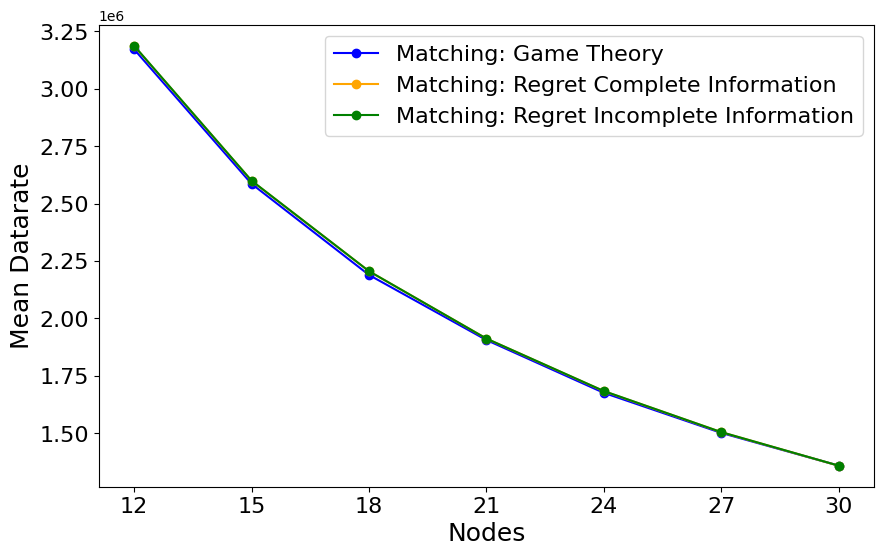
\includegraphics[width=\textwidth]{figures/chapter4/Mean_Datarate_vs_Users.png}
    \caption{Μέση ροή δεδομένων ανά αριθμό κόμβων ανά αλγόριθμο αντιστοίχισης}
    \label{fig7}
\end{figure}

Όπως φαίνεται στο \ref{fig7} ο αλγόριθμος Θεωρίας Παιγνίων πετυχαίνει την καλύτερη ροή δεδομένων ακολουθούμενος από τους Αλγορίθμους Ενισχυτικής Μάθησης και τέλος από την Τυχαία αντιστοίχιση. Παρατηρούμε πως όσο αυξάνεται ο αριθμός των κόμβων, η ροή δεδομένων μειώνεται, αφού περισσότεροι κόμβοι ανταγωνίζονται για τους διαθέσιμους πόρους κάθε εξυπηρετητή (εύρος ζώνης). Συνεπώς, όσο περισσότερους κόμβους έχουμε στο σύστημά μας τόσο λιγότερα δεδομένα μπορούν να στείλουν ταυτόχρονα στον κοινό εξυπηρετητή τους.

\begin{figure}[ht]
    \centering
    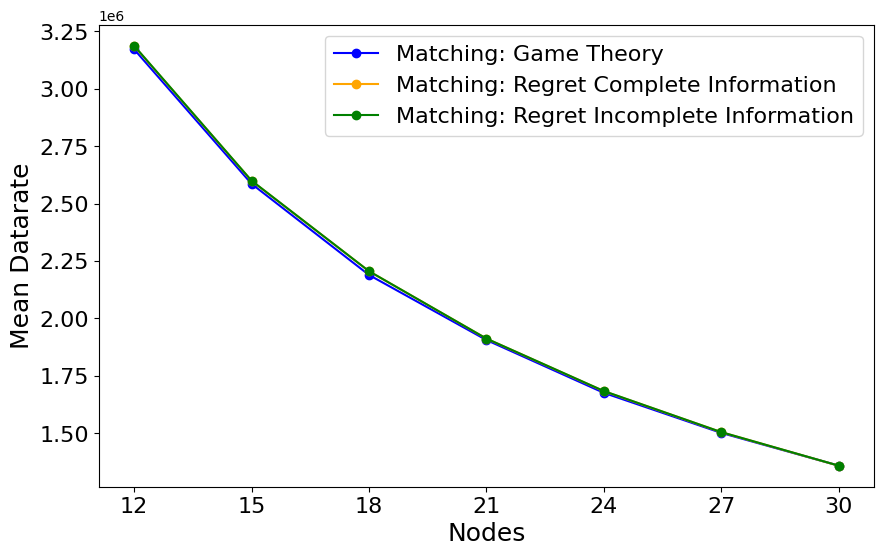
\includegraphics[width=\textwidth]{figures/chapter4/Mean_Datarate_vs_Users.png}
    \caption{Μέση ενέργεια μετάδοσης ανά αριθμό κόμβων ανά αλγόριθμο αντιστοίχισης}
    \label{fig8}
\end{figure}

Όπως είναι εμφανές στο διάγραμμα \ref{fig8}, όσο περισσότερους κόμβους έχουμε, αυτοί ανταγωνίζονται για περισσότερους πόρους και άρα η μέση ενέργεια μετάδοσης αυξάνεται. Όμως, βλέπουμε πως ο αλγόριθμος Θεωρίας Παιγνίων καταφέρνει και κρατά την ενέργεια αυτή χαμηλότερα απ' ότι οι υπόλοιπες λύσεις.

Αντίστοιχα στο διάγραμμα \ref{fig9}, παίρνοντας μετρήσεις για την μέση χρησιμότητα των κόμβων, αυτή σταδιακά μειώνεται όσο ο αριθμός των κόμβων αυξάνεται, επειδή και πάλι έχουμε ανταγωνισμό μεταξύ τους. Και σε αυτή τη μέτρηση όμως, ο αλγόριθμος Θεωρίας Παιγνίων πετυχαίνει το καλύτερο αποτέλεσμα.

\newpage

\begin{figure}[H]
    \centering
    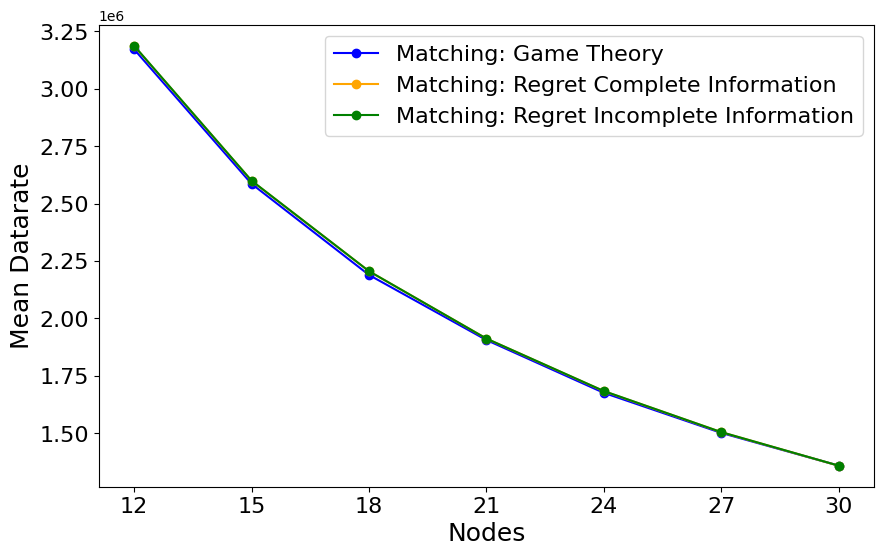
\includegraphics[width=\textwidth]{figures/chapter4/Mean_Datarate_vs_Users.png}
    \caption{Μέση χρησιμότητα κόμβων ανά αριθμό κόμβων ανά αλγόριθμο αντιστοίχισης}
    \label{fig9}
\end{figure}

\begin{figure}[H]
    \centering
    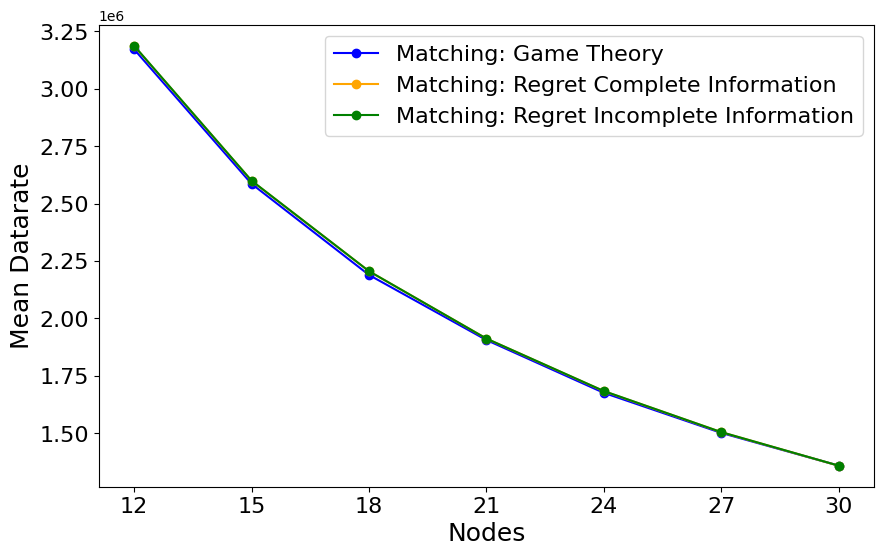
\includegraphics[width=\textwidth]{figures/chapter4/Mean_Datarate_vs_Users.png}
    \caption{Μέση χρησιμότητα εξυπηρετητών ανά αριθμό κόμβων ανά αλγόριθμο αντιστοίχισης}
    \label{fig10}
\end{figure}

\newpage

Αντίθετα στο διάγραμμα \ref{fig10}, η μέση χρησιμότητα των εξυπηρετητών αυξάνεται όσο περισσότεροι κόμβοι εισέρχονται στο σύστημά μας, αφού κάθε συμμαχία διαθέτει περισσότερους κόμβους και άρα περισσότερη πληροφορία. Ο αλγόριθμος Θεωρίας Παιγνίων και εδώ φαίνεται να κάνει τις καλύτερες αντιστοιχίσεις.

\begin{figure}[ht]
    \centering
    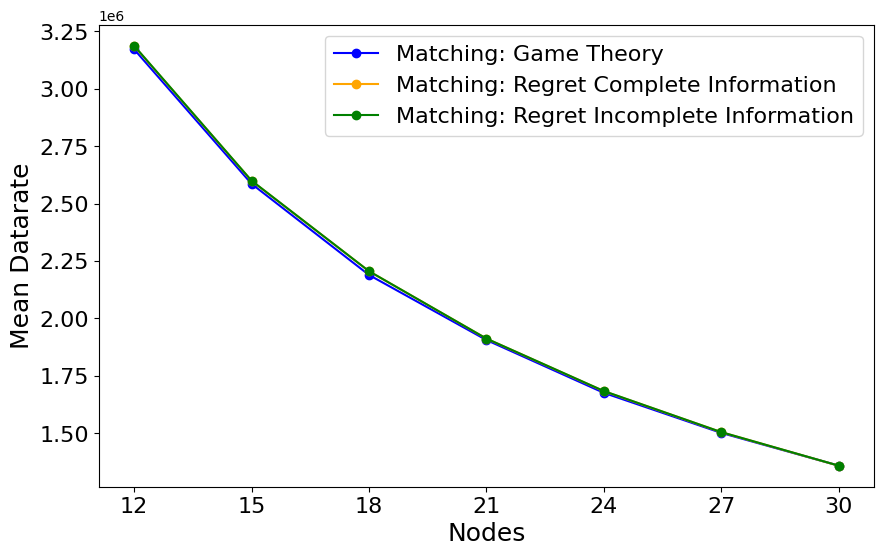
\includegraphics[width=\textwidth]{figures/chapter4/Mean_Datarate_vs_Users.png}
    \caption{Μέσος χρόνος εκτέλεσης ανά αριθμό κόμβων ανά αλγόριθμο αντιστοίχισης}
    \label{fig11}
\end{figure}

Προφανώς όσο περισσότερους κόμβους έχουμε στο σύστημά μας τόσο πιο δύσκολο θα είναι για τους αλγορίθμους μας να κάνουν την αντιστοίχισή τους στους εξυπηρετητές. Βλέποντας τα δεδομένα στο διάγραμμα \ref{fig11}, ο πιο γρήγορος αλγόριθμος είναι ο αλγόριθμος Τυχαίας Αντιστοίχισης, αφού είναι και ο πιο απλός. Από τους υπόλοιπους, ο αλγόριθμος Θεωρίας Παιγνίων επιτυγχάνει την πιο γρήγορη αντιστοίχιση, ακολουθούμενος από τους Αλγορίθμους Ενισχυτικής Μάθησης.

Παρακάτω παρουσιάζουμε τις συνολικές διαφορές σε όλα τα πειράματα που έγιναν μεταξύ των διάφορων αλγορίθμων.

Όπως φαίνεται στο διάγραμμα \ref*{fig12} ο αλγόριθμος Θεωρίας Παιγνίων πετυχαίνει κατά μέσο όρο το καλύτερο αποτέλεσμα όσον αφορά τη ροή δεδομένων από τους κόμβους στους εξυπηρετητές. Ελάχιστα χειρότερο αποτέλεσμα πετυχαίνει ο αλγόριθμος Ενισχυτικής Μάθησης ως προς χρησιμότητα κόμβων, ενώ ο αλγόριθμος Ενισχυτικής Μάθησης ως προς χρησιμότητα εξυπηρετητών και η Τυχαία Αντιστοίχιση πετυχαίνουν ακόμα χειρότερες λύσεις.

\newpage

\begin{figure}[H]
    \centering
    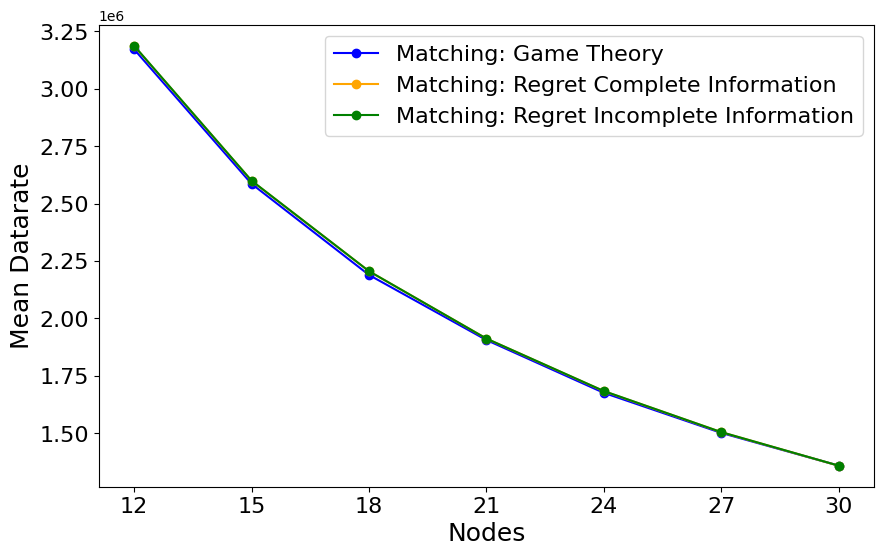
\includegraphics[width=\textwidth]{figures/chapter4/Mean_Datarate_vs_Users.png}
    \caption{Μέση ροή δεδομένων ανά αλγόριθμο αντιστοίχισης}
    \label{fig12}
\end{figure}

\begin{figure}[H]
    \centering
    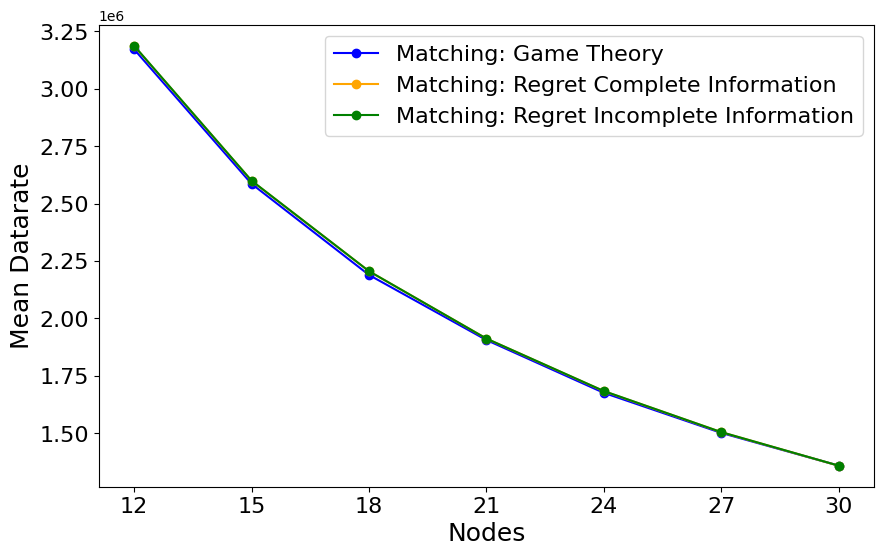
\includegraphics[width=\textwidth]{figures/chapter4/Mean_Datarate_vs_Users.png}
    \caption{Μέση ενέργεια μετάδοσης ανά αλγόριθμο αντιστοίχισης}
    \label{fig13}
\end{figure}

Στο διάγραμμα \ref*{fig13} βλέπουμε τις επιδόσεις των αλγορίθμων αναφορικά με τη μέση ενέργεια μετάδοσης που απαιτείται για την αποστολή των παραμέτρων των τοπικών μοντέλων στους εξυπηρετητές. Και πάλι ο αλγόριθμος Θεωρίας Παιγνίων πετυχαίνει το καλύτερο αποτέλεσμα, με τον αλγόριθμο Ενισχυτικής Μάθησης ως προς χρησιμότητα κόμβων να έχει πολύ κοντινή επίδοση. 

\begin{figure}[H]
    \centering
    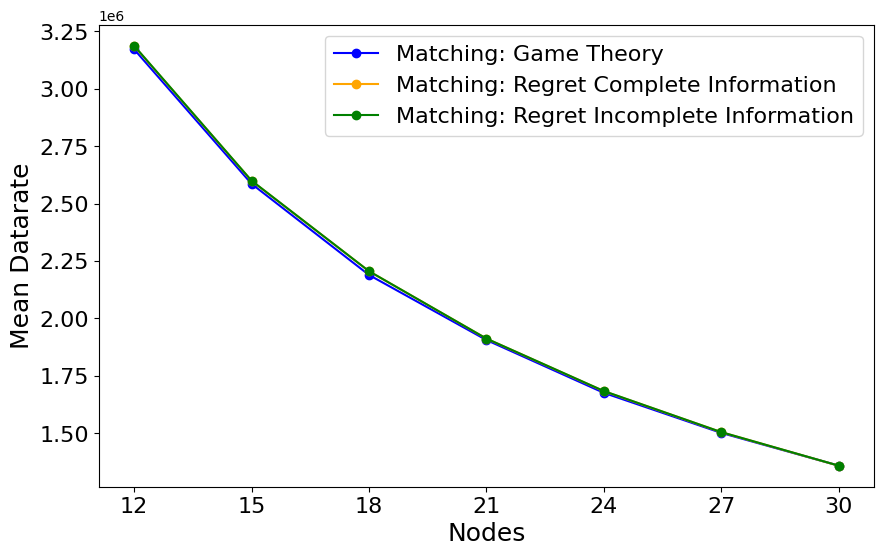
\includegraphics[width=\textwidth]{figures/chapter4/Mean_Datarate_vs_Users.png}
    \caption{Μέση χρησιμότητα κόμβων ανά αλγόριθμο αντιστοίχισης}
    \label{fig14}
\end{figure}

\begin{figure}[H]
    \centering
    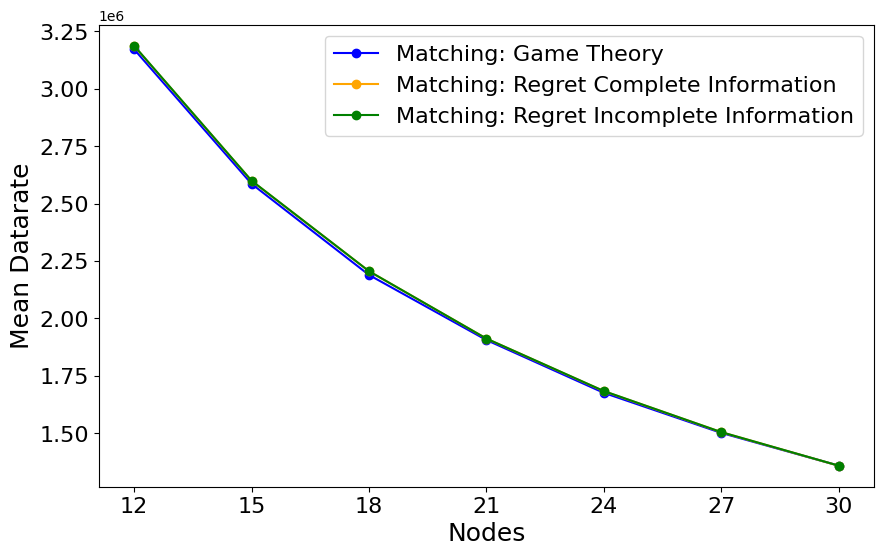
\includegraphics[width=\textwidth]{figures/chapter4/Mean_Datarate_vs_Users.png}
    \caption{Μέση χρησιμότητα εξυπηρετητών ανά αλγόριθμο αντιστοίχισης}
    \label{fig15}
\end{figure}

Αντίστοιχα στα διαγράμματα \ref*{fig14} και \ref*{fig15}, μπορούμε να δούμε πώς ο αλγόριθμος Θεωρίας Παιγνίων έχει την καλύτερη επίδοση όσον αφορά τις χρησιμότητες κόμβων και εξυπηρετητών. Με σειρά ακολουθούν ο αλγόριθμος Ενισχυτικής Μάθησης ως προς χρησιμότητα κόμβων, ο αλγόριθμος Ενισχυτικής Μάθησης ως προς χρησιμότητα εξυπηρετητών και τέλος η Τυχαία Αντιστοίχιση. Η σύγκριση στα δύο αυτά διαγράμματα αποτελεί ίσως την πιο σημαντική σύγκριση, αφού όλες οι αποφάσεις για την αντιστοίχιση παίρνονται ώστε να μεγιστοποιηθούν οι χρησιμότητες. Έτσι εδώ φαίνεται ξεκάθαρα η υπεροχή του αλγορίθμου Θεωρίας Παιγνίων έναντι των υπολοίπων.

Όσον αφορά τον χρόνο εκτέλεσης της αντιστοίχισης για τους αλγορίθμους μας,στο διάγραμμα \ref{fig16} βλέπουμε πως η Τυχαία Αντιστοίχιση προφανώς διαθέτει τον πιο γρήγορο μηχανισμό, ακολουθούμενη από τον αλγόριθμο Θεωρίας Παιγνίων και τέλος από τους αλγορίθμους Ενισχυτικής Μάθησης.

\begin{figure}[ht]
    \centering
    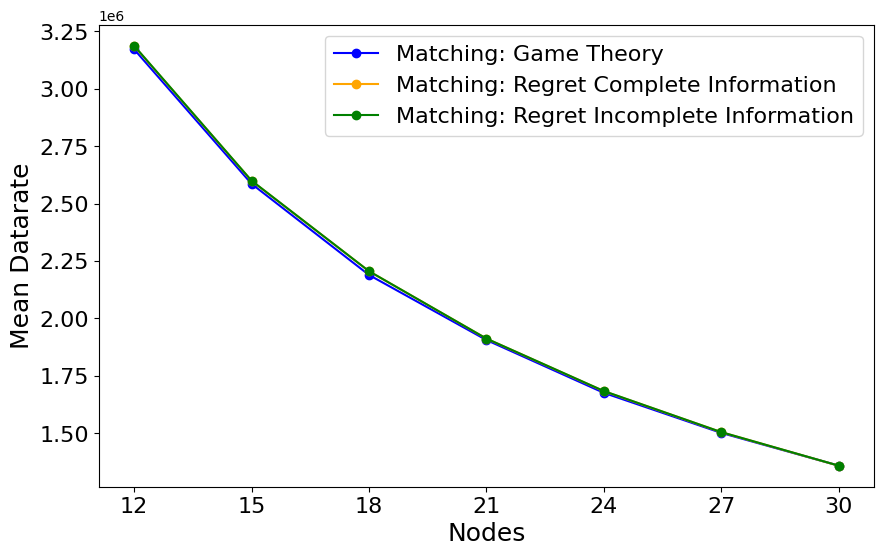
\includegraphics[width=\textwidth]{figures/chapter4/Mean_Datarate_vs_Users.png}
    \caption{Μέσος χρόνος εκτέλεσης ανά αλγόριθμο αντιστοίχισης}
    \label{fig16}
\end{figure}

\newpage

\begin{figure}[H]
    \centering
    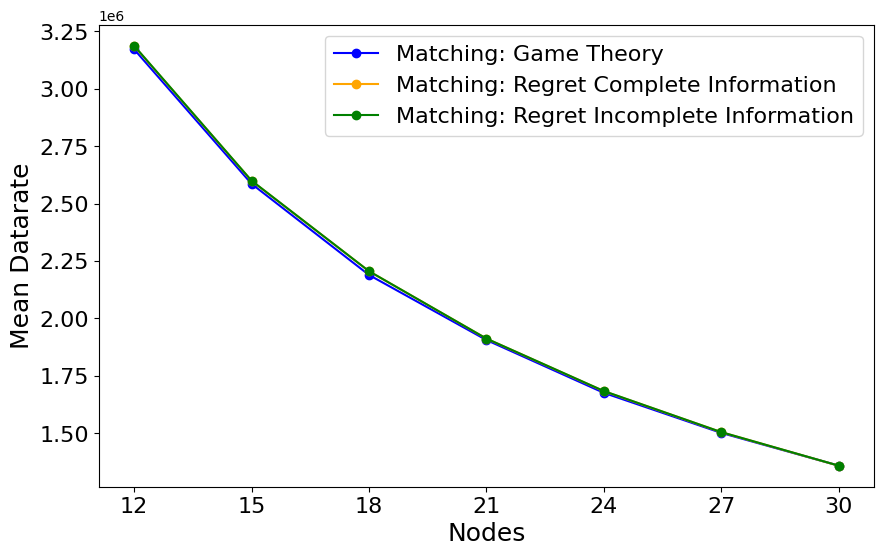
\includegraphics[width=\textwidth]{figures/chapter4/Mean_Datarate_vs_Users.png}
    \caption{Μέση ακρίβεια εξυπηρετητών (ανά καταστροφή) για κάθε αλγόριθμο αντιστοίχισης}
    \label{fig50}
\end{figure}

\begin{figure}[H]
    \centering
    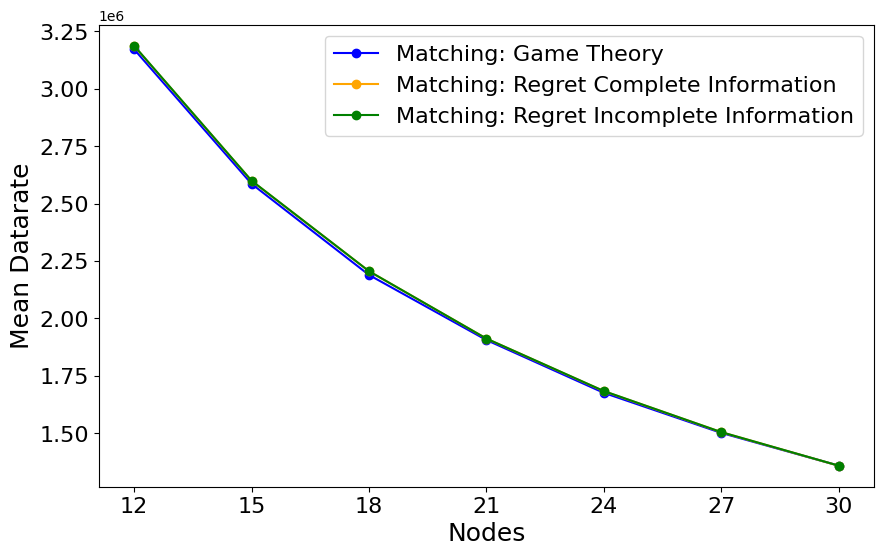
\includegraphics[width=\textwidth]{figures/chapter4/Mean_Datarate_vs_Users.png}
    \caption{Μέση απώλεια εξυπηρετητών (ανά καταστροφή) για κάθε αλγόριθμο αντιστοίχισης}
    \label{fig51}
\end{figure}

\newpage

Για την επίδοση των αλγορίθμων αντιστοίχισης ως προς την Ομοσπονδιακή Μάθηση, θα πρέπει να εξετάσουμε την ακρίβεια και την απώλεια που πετυχαίνουν, όπως αυτές φαίνονται στα διαγράμματα \ref*{fig50} και \ref*{fig51}. Ο αλγόριθμος Θεωρίας Παιγνίων καταφέρνει κατά μέσο όρο να έχει την μικρότερη απώλεια στους τρεις εξυπηρετητές του, ακολουθούμενος από τον αλγόριθμο Ενισχυτικής Μάθησης ως προς χρησιμότητα κόμβων. Είναι αξιοσημείωτο πως η Τυχαία Αντιστοίχιση παραμένει σχετικά κοντά στους αλγορίθμους μας, παρότι είναι το σημείο αναφοράς μας. Αυτό συμβαίνει επειδή στη διαδικασία της Ομοσπονδιακής Μάθησης συμπεριλαμβάνουμε έναν μηχανισμό ανάθεσης βαρών στους κόμβους μας, ανάλογα με την πληροφορία που διαθέτουν για τον εξυπηρετητή που έχουν συνδεθεί. Έτσι, κόμβοι με λίγη (ή και καθόλου χρήσιμη) πληροφορία θα επηρεάσουν πολύ λίγο την εκμάθηση του μοντέλου. Σε συνδυασμό με την πληροφορία που διαθέτει ο κάθε εξυπηρετητής, η Τυχαία Αντιστοίχιση επιτυγχάνει σεβαστές επιδόσεις παρά την απλότητα της. 